% Shared paper body.
\title{GROVE: Reusing Solution Sketches\\for Current-Flow Group Selection\iffull\\{\large(With Proof Appendices)}\fi}
\author{
\IEEEauthorblockN{Bowen Xue\IEEEauthorrefmark{1}, Tianyi Chen\IEEEauthorrefmark{1}, Xuanning Zeng\IEEEauthorrefmark{1}, Zifeng Peng\IEEEauthorrefmark{1}, Qiao Qi\IEEEauthorrefmark{1}\IEEEauthorrefmark{3}, Yongtai Liu\IEEEauthorrefmark{2}\IEEEauthorrefmark{3}}
\IEEEauthorblockA{
\IEEEauthorrefmark{1}Hangzhou Normal University, Hangzhou, China\\
\IEEEauthorrefmark{2}Hanyang University, Republic of Korea\\
\texttt{15869667756@163.com, hi@tychen.cc, zengxuanning49@gmail.com}\\
\texttt{p1057947506@163.com, qiqiao@hznu.edu.cn}\IEEEauthorrefmark{3}\texttt{, yt2024259263@hanyang.ac.kr}\IEEEauthorrefmark{3} (\IEEEauthorrefmark{3}corresponding authors)}
}
\maketitle
\begin{abstract}
Current-flow group closeness centrality (CFCC) selects network anchors
by minimizing the grounded Laplacian inverse trace. Greedy optimization
must re-estimate every remaining vertex's marginal contribution after
each selection. Rebuilding the estimates every round repeats expensive
batches of solves; caching them once and correcting them algebraically
is cheap, but its relative errors grow as the estimated quantities
shrink. We present \alg{}, which maintains two solution sketches of
the current grounded inverse through rank-one updates and, for
refreshed candidates, retains inverse moments obtained from individual
numerical solves; a per-round cap limits refreshes.
A uniform concentration argument, combined with residual bounds,
yields a $(1-1/e-\epsilon)$ approximation to optimal gain relative
to a fixed seed under explicit sketch and residual conditions, for
accuracy parameter $\epsilon>0$. On six graphs with completed comparisons, \alg{}
is $1.1$--$5.7\times$ faster than ApproxGreedy in the main runs, and
$1.4$--$3.8\times$ faster in four-seed means on four graphs. Final
inverse traces differ by at most 1.6\% across the compared methods;
the forest methods reach lower traces on roadNet-PA, and the
smallest-eigenvalue heuristic of Zhou et al.\ is faster on DBLP.
The cached shortcut ends 13.5\% higher in inverse trace than \alg{}
on roadNet-PA, at $2.5\times$ the time.
On LiveJournal, with 4.0 million vertices, \alg{} finishes in 4626
seconds. Supporting structural results cover completely monotone
grounding objectives, and inverse-power experiments characterize the
tradeoff between aggregate resistance and slow spectral modes.
\end{abstract}
\begin{IEEEkeywords}
Group centrality, node grounding, completely monotone functions,
supermodular optimization, randomized sketches, incremental computation.
\end{IEEEkeywords}

\section{Introduction}\label{sec:intro}
Resource placement and leader
selection~\cite{patterson2010,clark2014,lin2014} require groups of
vertices whose collective influence depends on paths throughout a
network.
Current-flow group closeness centrality (CFCC) measures this influence
through effective resistance~\cite{li2019}. Let $G=(V,E)$ be a
connected undirected graph with $n=|V|$ vertices and Laplacian $L$.
For a nonempty anchor set $S\subseteq V$, let
$L_{-S}=L[V\setminus S,V\setminus S]$ be its grounded principal
submatrix. Maximizing $\CFCC(S)=n/\tr(L_{-S}^{-1})$ is equivalent
to minimizing the total effective resistance to the anchors.

The computational bottleneck lies in choosing each additional anchor.
Greedy selection compares how much grounding each remaining vertex
decreases the inverse trace, and these marginal gains change after
every selection. ApproxGreedy estimates them through random
projections and Laplacian solves~\cite{li2019}; forest-based methods
use sampled spanning forests~\cite{xia2025}. Although each round
adds only one vertex, both repeat all-candidate estimation for the
updated grounded system. The central question is how to reuse this
work without letting stale estimates misdirect later choices.

Two natural approaches expose the difficulty. Rebuilding solution
sketches every round estimates the current matrix but repeats expensive
batches of solves. Alternatively, a scalar cache estimates each
candidate's moments---its inverse diagonal and squared inverse-column
norm---once, then subtracts algebraic decrements after each selection.
The initial sketch error persists in absolute terms. As true moments
shrink, their relative errors grow and may distort the ranking, and
the cache gives no way to tell beforehand on which inputs this happens.
The shortcut is competitive on most graphs we test, but on roadNet-PA
it ends with a 13.5\% higher inverse trace at $2.5\times$ the time of
our method.

\alg{} combines two forms of reuse. It maintains two solution sketches
of the current grounded inverse, updating them through rank-one
identities rather than rebuilding them through solves. Unrefreshed
candidates use these current sketches. Refreshed candidates instead
retain moments obtained from individual numerical solves.
Unlike the scalar-cache shortcut, this second path starts from a
solved column rather than a noisy initial sketch: exact decrements
preserve exact moments in exact arithmetic, and residual bounds
control the numerical implementation. A per-round refresh cap limits
additional candidate solves. The resulting algorithm maintains current
estimates while preserving work already spent on accurate candidates.

Reuse creates an adaptive estimation problem: selected vertices
depend on the same randomness used in subsequent rounds. We cover
all feasible grounding sets in one concentration event and combine it
with numerical-error bounds. For a fixed seed $S_0$, $k$ additional
anchors, and accuracy parameter $\epsilon>0$, sufficient sketch and
residual conditions yield a $(1-1/e-\epsilon)$ approximation to the
optimal gain relative to $S_0$. These are conservative worst-case
conditions; the practical sketch dimension of $d=64$ is evaluated
empirically. Our work bound separately accounts for sketch updates
and candidate refreshes.

We evaluate \alg{} on seven SNAP networks~\cite{snap2014} against
ApproxGreedy, our implementations of ForestCFCM and SchurCFCM, and
Zhou's smallest-eigenvalue heuristic~\cite{zhou2023}.
Matched comparisons, runtime components, ablations, parameter sweeps,
and additional random seeds test selection cost and quality.
The results show substantial savings on several graphs, a smaller
advantage on web-Google, and small quality tradeoffs rather than
uniform dominance. The largest completed input has about four million
vertices.

CFCC and the smallest grounded eigenvalue targeted by Zhou's
heuristic are usually treated as separate objectives. As a supporting
extension, completely monotone (CM) trace objectives place them in one
family. Hard-CFCC supermodularity and hardness are already
known~\cite{li2019}; our structural result covers all inverse powers
and heat traces under grounding. Increasing the inverse exponent
emphasizes slower modes. In separate exact-marginal experiments,
raising it from 1 to 4 increases the smallest grounded eigenvalue by
$1.51$--$2.33\times$ while the inverse trace rises by at most 0.60\%.

\smallskip\noindent\textbf{Contributions.}
\begin{enumerate}[leftmargin=*,itemsep=2pt,topsep=3pt]
\item \textbf{Hybrid CFCC selection.} Maintained solution sketches,
retained refreshed moments, and capped refresh reduce repeated
marginal-estimation work.
\item \textbf{Approximation and work.} A uniform adaptive event and
numerical-error budgets give a conditional seeded-gain guarantee,
with explicit refresh-sensitive costs.
\item \textbf{Evaluation and objective extensions.} Same-machine
comparisons and component measurements assess the reuse mechanism;
CM grounding structure and integer-power experiments explain the
separate spectral-weighting option.
\end{enumerate}

\section{Problem and Preliminaries}\label{sec:prelim}
Table~\ref{tab:notation} collects shared notation.
\subsection{Grounding queries}
Let $G=(V,E,w)$ be an undirected weighted graph with $n=|V|$
vertices and $m=|E|$ edges. Its nonnegative weights satisfy
$w_{ij}=w_{ji}$, with $w_{ij}=0$ for nonedges. The Laplacian has
entries $L_{ii}=\sum_jw_{ij}$ and $L_{ij}=-w_{ij}$ for $i\ne j$.
Write $M=L+\sigma I$, where $I$ is the identity and $\sigma\geq0$
is a uniform regularization parameter. For a selected set $S\subseteq V$,
let $\ind_S$ be its indicator vector and $\diag(\ind_S)$ the
matrix with this vector on the diagonal. A grounding penalty
$\beta\in(0,\infty]$ defines
\begin{equation}\label{eq:mainmatrices}
 A_S^\beta=
 \begin{cases}M+\beta\diag(\ind_S),&\beta<\infty,\\
 M[V\setminus S,V\setminus S],&\beta=\infty.
 \end{cases}
\end{equation}
Finite $\beta$ penalizes the selected vertices (soft grounding);
hard grounding removes their rows and columns. Write
$X_S=A_S^\infty$ for this active principal submatrix.
When $\sigma=0$, assume connectivity and a nonempty fixed seed
$S_0$; when $\sigma>0$, an empty seed is admissible.
We consider supersets of $S_0$, whose nonempty grounded matrices
are positive definite. The trace of a function of the empty matrix
is defined as zero.

A finite-valued function $f:(0,\infty)\to[0,\infty)$ is
\emph{completely monotone} (CM) if it admits the representation
\begin{equation}\label{eq:maincmrep}
 f(x)=\int_{[0,\infty)}e^{-tx}\,\mu(dt),\qquad \mu\geq0,
\end{equation}
where $\mu$ is a nonnegative measure on $[0,\infty)$ and $t$
is the integration variable. The matrix function applies $f$ to
each eigenvalue. The algorithmic target is hard CFCC:
$\beta=\infty$, $\sigma=0$, and $f(x)=x^{-1}$; the other
choices support the structural extension. Starting from $S_0$,
we select $k$ additional anchors:
\begin{equation}\label{eq:mainquery}
 \min_{T\subseteq V\setminus S_0,\ |T|=k}\Phi_f(S_0\cup T),
 \qquad \Phi_f(S)=\tr f(A_S^\beta).
\end{equation}
The \emph{seeded gain}, normalized relative to $S_0$, is
$F_f(T)=\Phi_f(S_0)-\Phi_f(S_0\cup T)$; its maximum over feasible
$k$-element extensions is $\OPT_k$. All approximation factors below
compare extensions of this same seed. The experimental total budget
is $K=|S_0|+k$: one seed and $K=20$ total anchors mean $k=19$
additions.

For a candidate $v\notin S$, its marginal cost reduction is
$\Delta_f(v\mid S)=\Phi_f(S)-\Phi_f(S\cup\{v\})$.
Supermodularity means
$\Delta_f(v\mid S)\geq\Delta_f(v\mid U)$ whenever
$S\subseteq U$ and $v\notin U$. Thus the seeded gain is
submodular; when it is also monotone, exact greedy selection achieves
the standard $1-1/e$ approximation to $\OPT_k$~\cite{nemhauser1978}.

\begin{table*}[t]
\centering\footnotesize
\caption{Notation shared across sections. Auxiliary proof variables are
local to their statements.}\label{tab:notation}
\begin{tabularx}{\textwidth}{@{}lXlX@{}}\toprule
Symbol & Meaning & Symbol & Meaning\\\midrule
$L,M$ & Laplacian and $M=L+\sigma I$ & $s,p$ & Real inverse exponent and positive integer exponent\\
$S_0,N$ & Fixed seed and $N=n-|S_0|$ initial candidates & $\Phi_s^0$ & Initial inverse-power cost $\Phi_s(S_0)$\\
$T,k,K$ & Added anchors, additional budget, total budget & $\Omega(u,v)$ & Pairwise effective resistance\\
$A_0,C,R_T$ & Seed matrix, incidence factor, current padded inverse & $Y_1,Y_2$ & CFCC solution sketches for first/second moments\\
$\Pi_C,\Pi_I$ & Independent random projection matrices & $\epsilon,\epsilon_{\rm forest}$ & GROVE accuracy parameter and forest-method input\\
$e_u,r_j(u,T)$ & Coordinate vector and $e_u^\top R_T^j e_u$ & $\bar R_v,s_x$ & Inverse after selecting $v$, and $\|Re_v\|^2$\\
$d,B_{\rm init},B_r,b_r$ & Sketch rows, initial/refresh batch widths, refresh cap & $\theta,\zeta,\delta$ & Acceptance, moment-error, and failure tolerances\\
$n_{\rm ref},n_t^{\rm ref}$ & Distinct refreshed candidates in total/in round $t$ & $\alpha_{\rm step},\alpha_{\rm cost}$ & Greedy-step fraction and trace-cost factor\\
$B_0,B_U$ & Seed approximate inverse and active restriction & $\mathcal E,\rho_{\rm res}$ & Sketch-error matrix and column-residual bound\\
$F_c,\mathcal T_t$ & Factor entries and work of a solve in round $t$ & $z_{\rm ser},\vartheta$ & Formal-series variable and removal interpolation\\
\bottomrule\end{tabularx}
\end{table*}

\subsection{Current flow and spectral weighting}
For hard grounding with $\sigma=0$, injecting one unit of current
at an ungrounded vertex $u$ produces voltage $(L_{-S}^{-1})_{uu}$
at $u$, equal to its effective resistance to the grounded set.
Summing these resistances gives the denominator of
CFCC~\cite{li2019}, so minimizing $\Phi_1(S)=\tr L_{-S}^{-1}$
maximizes CFCC.

More generally, inverse powers $f(x)=x^{-s}$, $s>0$, give
$\Phi_s(S)=\tr(A_S^\beta)^{-s}$. If $\lambda_i$ are the
positive eigenvalues of $A_S^\beta$, then
$\Phi_s(S)=\sum_i\lambda_i^{-s}$. For $\lambda_i<\lambda_j$,
their relative weights are $(\lambda_j/\lambda_i)^s$;
increasing $s$ therefore emphasizes slower spectral modes.
Heat instead weights each mode by $e^{-\tau\lambda_i}$ at horizon
$\tau>0$. CFCC is our main computational and experimental objective.
The broader family provides interpretable spectral weights.

The hard-grounding CFCC cost $\Phi_1$ is nonincreasing and
supermodular, and exact group selection is NP-hard~\cite{li2019}.
These known properties are all that the greedy algorithm and its
analysis in Sections~\ref{sec:algorithm} and~\ref{sec:analysis}
require; Section~\ref{sec:extensions} extends them to the CM family.

\begin{figure*}[t]
\centering
\begin{tikzpicture}[font=\footnotesize,>=Stealth,
  vtx/.style={circle,draw,fill=white,minimum size=9pt,inner sep=0pt},
  anc/.style={rectangle,draw,fill=black!75,minimum size=8pt,inner sep=0pt},
  can/.style={rectangle,draw,fill=black!25,minimum size=8pt,inner sep=0pt},
  box/.style={draw,rounded corners=2pt,align=center,inner sep=3pt,fill=black!3}]
% (a) coupling
\begin{scope}[scale=1.08]
\node[vtx,label={[font=\scriptsize]below:$i$}] (i) at (0,0) {};
\node[vtx] (a) at (1.1,0.55) {};
\node[vtx] (b) at (1.1,-0.55) {};
\node[anc,label={[font=\scriptsize]above:$S$}] (s1) at (2.3,0.75) {};
\node[can,label={[font=\scriptsize]below:$v$}] (v) at (2.3,-0.65) {};
\node[vtx] (c) at (3.3,0.05) {};
\node[anc,label={[font=\scriptsize]above:$S$}] (s2) at (4.3,0.05) {};
\foreach \x/\y in {i/a,i/b,a/b,a/s1,b/v,s1/c,v/c,c/s2} \draw[black!45] (\x)--(\y);
\draw[->,thick,blue!60!black,decorate,decoration={snake,amplitude=.6pt,segment length=5pt}]
  (i) to[bend left=12] (a);
\draw[->,thick,blue!60!black] (a) to[bend left=15] (b);
\draw[->,thick,blue!60!black] (b) to[bend left=10] (v);
\draw[->,thick,blue!60!black,dashed] (v) to[bend left=25] (i);
\node[align=center,font=\scriptsize] at (2.15,-1.45)
 {one walk for all sets; each anchor adds a killing clock;\\
  the extra loss from $v$ shrinks as $S$ grows};
\node[font=\small\bfseries] at (-0.3,1.15) {(a)};
\end{scope}
% (b) maintained state
\begin{scope}[xshift=6.5cm]
\node[box] (banks) at (0,0.55) {solution sketches\\$Y_1=\Pi_C C R,\ Y_2=\Pi_I R$};
\node[box] (ret) at (0,-0.75) {retained moments\\$r_1(u),\,r_2(u)$};
\node[box] (heap) at (3.35,-0.1) {heap of keys $r_2/r_1$\\sketch: unrefreshed\\retained: refreshed};
\node[box] (ref) at (6.45,-0.1) {refresh $\leq B_r$ per batch\\until tolerance $\theta$\\or cap $b_r$};
\node[box] (sel) at (9.35,-0.1) {select $v$\\$x=Re_v$\\$y=R^2e_v$};
\draw[->] (banks.east) -- (heap.west);
\draw[->] (ret.east) -- (heap.west);
\draw[->] (heap) -- (ref);
\draw[->] (ref) -- (sel);
\draw[->] (ref.south) |- node[below,font=\scriptsize,pos=.75]{refreshed values} ($(ret.east)+(0,-0.12)$);
\draw[->] (sel.north) |- node[above,font=\scriptsize,pos=.75]{rank-one solution sketch update \eqref{eq:mainbankupdate}} ($(banks.north)+(0,0.3)$) -- (banks.north);
\draw[->] (sel.south) |- node[below,font=\scriptsize,pos=.75]{exact decrements \eqref{eq:mainr1}--\eqref{eq:mainr2}} ($(ret.south)+(0,-0.35)$) -- (ret.south);
\node[font=\small\bfseries] at (-1.55,1.2) {(b)};
\end{scope}
\end{tikzpicture}
\caption{(a) The CM coupling: all grounding sets share one walk and one
family of killing clocks, so a new anchor removes fewer surviving
returns when more anchors are present. (b) The maintained state of
\alg{}: unrefreshed candidates are keyed from the current solution sketches,
refreshed candidates from retained exact moments; after each selection
both paths are updated from the selected inverse columns.}
\label{fig:overview}
\end{figure*}

\section{The Hybrid CFCC Algorithm}\label{sec:algorithm}
We now specialize to hard grounding with $\sigma=0$ and CFCC
($s=1$). To avoid rebuilding all marginal estimates after every
anchor, \alg{} maintains solution sketches for unrefreshed candidates
and scalar moments for candidates already refreshed by a solve.
The two paths preserve different information about the current matrix
(Fig.~\ref{fig:overview}(b)).

Let $W=V\setminus S_0$ contain the $N=n-|S_0|$ initial candidates.
The seed matrix is $A_0=L[W,W]=C^\top C\in\R^{N\times N}$,
where $C\in\R^{m\times N}$ is the oriented edge-incidence matrix,
scaled by square roots of edge weights and restricted to columns in
$W$. This exact incidence factor is distinct from the approximate
Cholesky factor used for preconditioning. For additional anchors
$T\subseteq W$, let $R_T$ be the current active inverse, embedded
in $\R^{N\times N}$ with zero rows and columns at $T$.
Write $R=R_T$, let $e_u$ be the coordinate unit vector at an active
candidate $u$, and define $r_j(u,T)=e_u^\top R_T^j e_u$ for
integer $j\geq1$. The CFCC marginal is
\begin{equation}\label{eq:ratio}
 \Delta_1(u\mid S_0\cup T)=\frac{r_2(u,T)}{r_1(u,T)},\qquad
 r_1=R_{uu},\quad r_2=\|Re_u\|^2.
\end{equation}
Here $\|\cdot\|$ is the Euclidean norm. Both moments come from
one inverse column, so a candidate refresh requires one solve
rather than two complete trace estimates.

\subsection{Common-seed initialization}
The initial anchor approximately minimizes $L^+_{vv}$, where $L^+$
is the Moore--Penrose pseudoinverse. Writing $\Omega(u,v)$ for
pairwise effective resistance, the identity
$\sum_u\Omega(u,v)=\tr L^++nL^+_{vv}$ gives the singleton
CFCC rule~\cite{li2019,xia2025}. We estimate this diagonal with
an incidence-based random-sign sketch, projecting right-hand sides
and solutions onto $\ind^\perp=\{x:\ind^\top x=0\}$, where
$\ind$ is the all-ones vector. Every compared method receives the
common seed $S_0=\{s_0\}$. Its computation is a separate shared
stage; all later gains use this seed as their fixed baseline.

Initializing scalar estimates once saves solves, but subtracting exact
decrements preserves their initial absolute error. As moments shrink,
this error can distort their ratios. \alg{} instead maintains
sketches of the \emph{current} inverse. Draw independent random
matrices $\Pi_C\in\R^{d\times m}$ and $\Pi_I\in\R^{d\times N}$ with
independent mean-zero entries of variance $1/d$. Starting at
$R=A_0^{-1}$, construct the two $d\times N$ solution sketches
\begin{equation}\label{eq:banks}
 Y_1=\Pi_C C R,\qquad Y_2=\Pi_I R,\qquad
 \widehat r_j(u)=\|Y_j[:,u]\|^2\quad(j=1,2).
\end{equation}
The notation $Y_j[:,u]$ denotes column $u$. The identity $RA_0R=R$
gives $\|CRe_u\|^2=r_1(u)$ and $\|Re_u\|^2=r_2(u)$, so the
squared column norms estimate the two current moments.
Initialization uses $d$ sparse-system right-hand sides per solution sketch.

\subsection{Two complementary update paths}
Grounding one vertex gives a rank-one inverse correction, which can
be applied directly to both solution sketches. An \emph{unrefreshed} candidate
uses the updated solution-sketch column norms. A \emph{refreshed}
candidate has undergone an individual solve and thereafter retains
its moments through scalar updates. The following identities describe
both paths in exact arithmetic.

\begin{proposition}[Hybrid state identities]\label{main:maintenance}
On selecting $v$, let $x=Re_v$, $y=R^2e_v$, $c=1/x_v$,
and $s_x=\|x\|^2$. The next inverse is
$R'=R-cxx^\top$, with a zero row and column at $v$.
Both solution sketches update as
\begin{equation}\label{eq:mainbankupdate}
 Y_j'=Y_j-cY_j[:,v]x^\top,\qquad j=1,2.
\end{equation}
For each remaining refreshed candidate $u$, retain its moments by
\begin{align}
 r_1'(u)&=r_1(u)-cx_u^2,\label{eq:mainr1}\\
 r_2'(u)&=r_2(u)-2cx_uy_u+c^2s_x x_u^2.\label{eq:mainr2}
\end{align}
With exact columns, exact refreshed moments remain exact. A scalar
cache initialized with error $e_j(u)$ retains that signed absolute
error under exact independent decrements.
The solution sketch update costs $O(Nd)$ work and storage; scalar retention
costs $O(N)$ work, once $x,y$ are available.
\end{proposition}
\begin{proof}[Proof sketch]
The principal-inverse identity gives $R'=R-cxx^\top$.
Multiplication by the fixed sketch factors gives
\eqref{eq:mainbankupdate}. Taking diagonals gives
\eqref{eq:mainr1}; squaring first gives \eqref{eq:mainr2}.
Subtracting the same decrement from a true moment and its cached
estimate preserves their signed difference.
\end{proof}

After each selection, \alg{} updates both solution sketches for all remaining
vertices and the scalar moments of refreshed candidates. Retention
allows a later round to choose an already refreshed candidate without
another refresh. A winning refresh provides $x$; the additional
column $y$ supports scalar maintenance. Both are reused when available.
Numerical solves introduce errors controlled by the tolerances below
and analyzed in Section~\ref{sec:analysis}.

\subsection{Capped candidate refresh}
At each round, rebuild a max-heap from the current moment ratios,
using solution sketch estimates for unrefreshed candidates and retained values
for refreshed ones. Refreshed heap tops update the incumbent without
a solve; unrefreshed candidates are refreshed in blocks of at most
$B_r$. Let $b$ be the best refreshed marginal found and $q_{\rm heap}$ the
largest remaining key. Stop when $b\geq(1-\theta)q_{\rm heap}$, with
acceptance tolerance $0\leq\theta<1$, or when the positive refresh
cap $b_r$ is reached. A zero cap means unlimited refreshes.
The cap controls candidate solves, not solution sketch maintenance. It is checked
between batches, so a positive cap can be exceeded by fewer than
$B_r$ refreshes; the initial maximum-key candidate is always processed
before a cap stop.

Algorithm~\ref{alg:grove} uses total budget $K$, initialization
batch width $B_{\rm init}$, and refresh batch width $B_r$.
The relative solve tolerances $\varepsilon_{\rm init},\varepsilon_{\rm ref},\varepsilon_{\rm upd}$ apply to
initialization, candidate refreshes, and newly computed update columns,
respectively. A reused winning column retains its $\varepsilon_{\rm ref}$ tolerance.
The seed preconditioner is constructed once and masked for later solves.

\begin{algorithm}[t]
\caption{\alg{}: hard-CFCC hybrid selection}\label{alg:grove}
\footnotesize
\textbf{Input:} $G$, common seed $s_0$, total budget $K$;
$d,B_{\rm init},B_r,b_r,\theta$; solve tolerances $\varepsilon_{\rm init},\varepsilon_{\rm ref},\varepsilon_{\rm upd}$.
\begin{enumerate}[leftmargin=1.8em,label=\arabic*.,itemsep=1pt,topsep=2pt]
\item Ground $s_0$; construct the seed preconditioner if enabled.
Initialize $Y_1,Y_2$ and moments using batches of width $B_{\rm init}$
and tolerance $\varepsilon_{\rm init}$. Mark all candidates unrefreshed.
\item For rounds $1,\ldots,K-1$:
\begin{enumerate}[leftmargin=1.5em,label=\alph*.,itemsep=1pt,topsep=1pt]
\item Build heap $\mathcal H$ with key $r_2(u)/r_1(u)$.
Set incumbent value $b=-\infty$, winner $v=\bot$, refresh count $r=0$.
\item Consume refreshed heap tops and update $(v,b)$ from their values.
Let $q_{\rm heap}$ be the largest remaining key, or $-\infty$ if empty.
\item If $v\ne\bot$ and $b\geq(1-\theta)q_{\rm heap}$, stop this round.
If $v\ne\bot$, $b_r>0$, and $r\geq b_r$, also stop.
\item Pop entries until up to $B_r$ unrefreshed candidates are collected;
refreshed entries encountered update the incumbent without a solve.
Refresh the collected candidates at $\varepsilon_{\rm ref}$, mark them refreshed,
update $(v,b)$, and retain a newly winning column $Re_v$.
Increase $r$ by the batch size and return to step 2b.
\item Before a nonfinal round ends, obtain $x=Re_v$ and $y=R^2e_v$.
Reuse a retained winning column when enabled; solve any missing
columns at $\varepsilon_{\rm upd}$.
Update both solution sketches by \eqref{eq:mainbankupdate}.
For unrefreshed candidates recompute moment norms; for refreshed
candidates apply \eqref{eq:mainr1}--\eqref{eq:mainr2}.
\item Zero coordinate $v$, add $v$ to the grounded set, and mask it
in subsequent solves. Skip maintenance after the final selection.
\end{enumerate}
\item Return the $K$ grounded nodes, including $s_0$.
\end{enumerate}
\end{algorithm}

Classical lazy greedy (CELF) reuses stale exact marginal upper bounds
from submodularity~\cite{leskovec2007}. A raw JL estimate is not such
an upper bound: combining ApproxGreedy with lazy ordering requires
calibrated intervals or fresh accuracy events. \alg{} instead updates
current estimates and retains individually refreshed moments; its
cap is analyzed on the uniform event in Section~\ref{sec:analysis}.
Two restrictions isolate the update paths in
Section~\ref{sec:experiments}. \emph{Sketch-only} maintains both
solution sketches but rekeys every candidate from them each round, removing the
retained scalar path and its $y$ solve. \emph{Scalar cache}
initializes moments once and applies algebraic decrements without
maintaining solution sketches. Their comparison tests whether current sketches
and retained values reduce different sources of repeated work.

\section{Approximation and Work}\label{sec:analysis}
Reuse saves solves but couples later choices to the original random
sketches. We first control this adaptivity, then incorporate numerical
errors, summarize the solver policy, and account for the work
that remains after eliminating repeated all-candidate solves.

\subsection{One event for adaptive selection}
Accuracy for a fixed matrix is insufficient when the selected anchors
depend on the sketches. We therefore cover every feasible grounding
set in one event. Let $\delta$ be its failure probability and
$\zeta$ the relative moment-error tolerance. The count $\mathcal N_{N,k}$
below includes every active candidate paired with a set of at most
$k$ added anchors; $\alpha_{\rm step}$ is the resulting per-round greedy factor.
\begin{theorem}[Adaptive hybrid guarantee]\label{main:guarantee}
Fix $S_0$, $1\leq k<N$ additions, $0<\delta,\zeta<1$, and define
\[
 \mathcal N_{N,k}=\sum_{t=0}^{k}\binom Nt(N-t),\qquad
 d\geq\left\lceil8\zeta^{-2}\log\frac{4\mathcal N_{N,k}}\delta\right\rceil.
\]
Use independent Gaussian entries of variance $1/d$, or independent
signs $\pm1/\sqrt d$, in the two solution sketches. With probability at least
$1-\delta$, exact maintenance gives relative error at most $\zeta$
for both moments at every active vertex of every $|T|\leq k$.
For exact refreshed values, put $\chi=(1+\zeta)/(1-\zeta)$ and
\[
 \alpha_{\rm step}=\min\{\chi^{-2},(1-\theta)\chi^{-1}\}.
\]
Algorithm~\ref{alg:grove}, with any positive cap or unlimited
refreshes, returns gain at least $(1-e^{-\alpha_{\rm step}})\OPT_k$.
In particular, $\zeta\leq\epsilon/8$ and
$\theta\leq\epsilon/2$ give $(1-1/e-\epsilon)\OPT_k$.
The sufficient dimension is
$O(\epsilon^{-2}((k+1)\log(N+1)+\log(1/\delta)))$.
\end{theorem}
\begin{proof}[Proof sketch]
\emph{One fixed column.} For a deterministic nonzero target vector
$w$ and one unscaled random sketch row $g$, the normalized projection
$Z=g^\top w/\|w\|$ satisfies $\E Z^2=1$ and
$\E e^{tZ}\leq e^{t^2/2}$ for both row distributions, hence
$\E e^{tZ^2}\leq(1-2t)^{-1/2}$ for $0<t<1/2$. A Chernoff bound on the
average of $d$ copies of $Z^2$ gives upper-tail failure at most
$e^{-d\zeta^2/8}$; the inequality $e^{-y}\leq1-y+y^2/2$ and
$\E Z^4\leq3$ give lower-tail failure at most $e^{-d\zeta^2/6}$.

\emph{All adaptive trajectories.} The targets $CR_Te_u$ and $R_Te_u$,
over all $|T|\leq k$ and active $u$, form a \emph{deterministic}
family of $2\mathcal N_{N,k}$ vectors. A union bound puts all of them inside
relative error $\zeta$ with probability at least $1-\delta$. The
maintained solution sketches equal $\Pi_C C R_T$ and $\Pi_I R_T$ exactly for whatever $T$ the
algorithm reaches, so adaptive selection, refresh patterns, and
stopping decisions stay on this event.

\emph{One round.} Write $\Delta_u$ for candidate $u$'s true
current marginal. Every key lies in $[\Delta_u/\chi,\chi\Delta_u]$,
and refreshed keys are exact. Let $u_*$ maximize $\Delta_u$, let $w$
carry the largest initial key, and retain the incumbent $b$ and
remaining maximum key $q_{\rm heap}$ from Algorithm~\ref{alg:grove}. At a cap
stop $w$ has been processed, so the incumbent satisfies
$b\geq\Delta_w\geq\mathrm{key}(w)/\chi\geq\Delta_{u_*}/\chi^2$. At an
acceptance stop, processed values are at most $b$ and an unprocessed
$u$ has $\Delta_u\leq\chi q_{\rm heap}\leq\chi b/(1-\theta)$; hence
$b\geq(1-\theta)\Delta_{u_*}/\chi$.

\emph{Greedy recurrence.} By monotonicity and supermodularity of the hard-CFCC
cost~\cite{li2019}, the gap to
$\OPT_k$ is at most $k$ times the largest marginal, so it contracts by
$1-\alpha_{\rm step}/k$ per round, giving $1-(1-\alpha_{\rm step}/k)^k\geq1-e^{-\alpha_{\rm step}}$.
Finally $1-\chi^{-2}\leq4\zeta$, $1-(1-\theta)\chi^{-1}\leq\theta+2\zeta$,
and $e^{-\alpha_{\rm step}}-e^{-1}\leq1-\alpha_{\rm step}$, while
$\mathcal N_{N,k}\leq(k+1)N^{k+1}$ yields the dimension order.
\end{proof}

The sufficient dimension records the price of adaptive reuse.
Fresh independent solution sketches require
$d_{\mathrm{fresh}}=\lceil8\zeta^{-2}\log(4Nk/\delta)\rceil$
for the corresponding ideal-solve event: each current matrix is fixed
conditional on preceding rounds. Maintained solution sketches instead cover all
feasible matrices at initialization. This extra dependence on $k$
trades a larger uniform-accuracy requirement for fewer repeated solves.

The bound is a worst-case sufficient condition. For example,
$\epsilon=0.5$, $\zeta=\epsilon/8$, $\delta=0.1$, and $k=19$
give $d\geq445{,}823$ at $N=317{,}079$ and
$d\geq492{,}870$ at $N=10^6$. Our experimental $d=64$ is an
empirical operating point, outside these sufficient-dimension
settings; Table~\ref{tab:dsweep} evaluates its accuracy--work tradeoff.

\subsection{Numerical accuracy}
Practical solves perturb both update paths. For a computed solution sketch
$\widetilde Y$ and its ideal counterpart $Y$, write
$\mathcal E=\widetilde Y-Y$ and measure the error by
$\|\mathcal E\|_{F,A_0}=\sqrt{\tr(\mathcal E A_0\mathcal E^\top)}$.
Let $e_1,e_2$ bound this norm for the first and second solution sketches.
Let $a>0$ and $B>0$ bound the smallest and largest eigenvalues
of $A_0$, respectively. The next result propagates a selected-column
residual into solution sketch and moment errors. Supported errors
and columns have zero coordinates at already grounded vertices.

\begin{proposition}[Residual-controlled maintenance]\label{main:residual}
Let $a\leq\lambda_{\min}(A_0)$ and
$B\geq\lambda_{\max}(A_0)$. Suppose a supported selected column
$\widetilde x$ has $\widetilde x_v>0$ and true active-system
residual norm at most $\rho_{\rm res}$. If a solution sketch's current error is at most
$e$ in $\|\mathcal E\|_{F,A_0}^2=\tr(\mathcal E A_0\mathcal E^\top)$, its update has error
at most
\begin{equation}\label{eq:mainresidual}
 e^+=e+\frac{\|\widetilde Y[:,v]\|\rho_{\rm res}}
                   {\sqrt a\,\widetilde x_v}+\omega,
\end{equation}
where $\omega$ bounds supported rounding error in the same norm.
On the ideal-sketch event with tolerance $\zeta_0$, the relative
moment errors are bounded by
\[
 \zeta_0+2\sqrt{1+\zeta_0}\,e_1+e_1^2,
 \quad
 \zeta_0+2\sqrt{1+\zeta_0}\sqrt B\,e_2+B e_2^2.
\]
Thus a target tolerance $\bar\zeta<1$ is met by
$\zeta_0=\bar\zeta/2$ and
$e_1,\sqrt B e_2\leq\bar\zeta/8$.
\end{proposition}
\begin{proof}[Proof sketch]
Let $U$ be the active coordinates, $x=R_Te_v$,
$h=\widetilde x-x$, and $\|w\|_{A_0}^2=w^\top A_0w$.
The residual gives $\|h\|_{A_0}\leq\rho_{\rm res}/\sqrt a$.
Active inverse equations give
$\langle h,x\rangle_{A_0}=h_v$ and $\|x\|_{A_0}^2=x_v$; hence
\[
 \left\|\frac{\widetilde x}{\widetilde x_v}-\frac{x}{x_v}\right\|_{A_0}^2
 =\frac{\|h\|_{A_0}^2-h_v^2/x_v}{\widetilde x_v^2}
 \leq\frac{\rho_{\rm res}^2}{a\widetilde x_v^2}.
\]
Put $P=I-e_vx^\top/x_v$ and $\mathcal E=\widetilde Y-Y$.
Expanding the supported-row energies yields
\[
 \|\mathcal E P\|_{F,A_0}^2
 =\|\mathcal E\|_{F,A_0}^2-\|\mathcal E[:,v]\|^2/x_v.
\]
The computed-minus-ideal update is
\begin{align*}
 \widetilde Y'-Y'={}&\mathcal E P+D_{\rm rnd}\\
 &+\widetilde Y[:,v]
       (x/x_v-\widetilde x/\widetilde x_v)^\top,
\end{align*}
where $\|D_{\rm rnd}\|_{F,A_0}\leq\omega$.
Contraction of $\mathcal E P$, the outer-product norm, and the
triangle inequality give \eqref{eq:mainresidual}.
For sketch $j$, the coordinate-representer bound is
$\|\mathcal E[:,u]\|\leq e_j\sqrt{r_1(u)}$.
For $Y_1$ this is relative to $\sqrt{r_1}$; for $Y_2$ use
$r_1\leq Br_2$. Expanding the perturbed squared norms on the
ideal-sketch event gives the two stated moment-error bounds.
\end{proof}

Retained scalar moments follow a separate error path: their refresh
error plus accumulated decrement-error bounds. The coefficients use
independently solved selected columns, so candidate-cache errors do
not feed back into them. To combine both paths, let $\nu<1$ bound
the relative error of computed refreshed marginals and let
$\bar\zeta<1$ be the target solution sketch-moment tolerance. Define
\[
 \eta=\max\left\{\frac{1+\bar\zeta}{1-\bar\zeta}-1,\nu\right\}<1.
\]
A sufficient inexact step factor is
\[
 \alpha_{\rm num}=\frac{1-\nu}{1+\nu}
 \min\left\{\frac{1-\eta}{1+\eta},(1-\theta)(1-\eta)\right\}.
\]
The minimum follows the two stopping cases in
Theorem~\ref{main:guarantee}; the prefactor accounts for choosing
the incumbent using approximate refreshed values.
Assigning sampling and numerical budgets so that
$\alpha_{\rm num}\geq1-\epsilon$ gives the stated
$(1-1/e-\epsilon)$ seeded-gain factor. Thus sketch concentration,
column residuals, and retained-moment errors enter one approximation
condition.

\subsection{Solver implementation}
\alg{} constructs an approximate-Cholesky seed preconditioner and
masks grounded coordinates in later applications. Blocks with fewer
than four right-hand sides use Jacobi preconditioning; on roadNet-PA
the seed factor is used for every block. This mixed solver policy is
part of the evaluated implementation.

For work accounting, suppose the seed approximate inverse $B_0$
satisfies $a_cA_0^{-1}\preceq B_0\preceq b_cA_0^{-1}$, with
$0<a_c\leq b_c$, and put $\chi_c=b_c/a_c$.
Here $P\preceq Q$ means $Q-P$ is positive semidefinite.
For active coordinates $U$ after $t$ additions, define
$A=A_0[U,U]$ and $B_U=B_0[U,U]$.
The preconditioned conjugate-gradient (PCG) error is measured in
$\|e_h\|_A=\sqrt{e_h^\top Ae_h}$, where $e_h$ is the solution
error after $h$ iterations. Under the stated seed-quality premise,
$t+O(\sqrt{\chi_c}\log(1/\xi))$ iterations suffice for relative
energy accuracy $\xi$, capped by $|U|$.
The block inverse formula gives
$(A_0^{-1})[U,U]=A^{-1}+ZZ^\top$, where the positive
Schur-complement correction has $\operatorname{rank}Z\leq t$.
After congruence by $A^{1/2}$, restricting the seed bounds shows
that $A^{1/2}B_UA^{1/2}$ has no eigenvalue below $a_c$ and at
most $t$ above $b_c$. A PCG residual polynomial places roots at
the large outliers and uses a Chebyshev factor on $[a_c,b_c]$.
The outlier factors have magnitude at most one on that interval.
For $\chi_c>1$ and $h\geq t$, this gives
\[
 \frac{\|e_h\|_A}{\|e_0\|_A}
 \leq2\left(\frac{\sqrt{\chi_c}-1}{\sqrt{\chi_c}+1}\right)^{h-t},
\]
which yields the iteration bound. For $\chi_c=1$, at most $t+1$
iterations suffice; the dimension cap is $|U|$ in either case.
The Kyng--Sachdeva construction~\cite{kyng2016} supplies one
admissible seed-quality guarantee. The implementation uses a lightweight
clique-sampling variant, with separate condition-number-dependent
bounds for its Jacobi calls.

\subsection{Work and comparison with fresh-round selection}
The work saved by reuse depends on how often solution sketch updates and
retained values replace candidate solves. Let $T_{\rm build}$ be
preconditioner construction work, $n_{\rm ref}$ the total number of
distinct refreshed candidates, $n_t^{\rm ref}$ the count in round $t$,
$F_c$ the number of stored factor entries, and $\mathcal T_t$ the
work of one solve at the required precision in that round.
The hybrid's work is
\begin{align}\label{eq:mainwork}
 T_{\rm build}+O\bigg(&dm+2d\mathcal T_0+
 \sum_{t=0}^{k-1}n_t^{\rm ref}\mathcal T_t+
 2\sum_{t=0}^{k-2}\mathcal T_t\\
 &+kNd+kN+(kn_{\rm ref}+n_{\rm ref}+k)\log(N+1)\bigg).\notag
\end{align}
The $dm$ term forms the incidence-based sketch right-hand sides,
and $2d\mathcal T_0$ covers initial solution sketch solves; the two sums
cover candidate refreshes and selected-column maintenance. Reusing
the winning column reduces the latter. The $kNd$ and $kN$ terms
cover solution sketch and scalar updates, respectively.
The solution sketches require $O(Nd)$ storage in addition to the graph,
factor, scalar moments, and solve batches. Exact retention makes
$n_{\rm ref}\leq N$; with a common positive cap and batch width,
$n_{\rm ref}\leq\min\{N,k(b_r+B_r-1)\}$.
The heap term covers previously refreshed candidates that are
processed again without a solve.

Under the preceding seed-quality premise, an all-factor
configuration can take
\[
 \mathcal T_t=O\bigl((m+N+F_c)
 \min\{N-t,t+1+\sqrt{\chi_c}\log(2/\xi)\}\bigr).
\]
Jacobi calls instead use their own condition-number-dependent
iteration bound. The maintained algorithm is nearly linear in graph
size for fixed budget, precision, and refresh parameters. Substituting
the uniform dimension into \eqref{eq:mainwork} exposes an array-update
term of order $\widetilde O(k^2N\epsilon^{-2})$, alongside
initialization and selected/refreshed solves.

At $s=1$, fresh-round JL selection with an SDDM solver has
$\widetilde O(km\epsilon^{-2})$ selection work, as in
ApproxGreedy~\cite{li2019,spielman2014}. This uses fresh
$O(\epsilon^{-2}\log(Nk/\delta))$-row sketches and accurate
solves in each round. In contrast, \eqref{eq:mainwork} retains
the maintained method's explicit budget, array-update, and refresh
costs; empirical savings arise when updates replace enough solves.

\section{Extension: Completely Monotone Objectives}\label{sec:extensions}
The CFCC algorithm uses only $s=1$ and the known hard-grounding
structure~\cite{li2019}. This section extends that structure to every
CM trace objective and supports the separate inverse-power experiment
in Section~\ref{sec:powers}. Positive integer powers $p\geq1$ provide
a tunable objective for exact-marginal selection on medium graphs,
allowing aggregate resistance and slow modes to receive different weights.

\subsection{CM grounding structure}\label{sec:structure}
The \emph{admissible lattice} is the family of sets containing the
fixed seed $S_0$; an \emph{available vertex} lies outside the
current selected set.

\begin{theorem}[CM grounding structure]\label{main:cm}
For every CM function $f$ and every $\beta\in(0,\infty]$,
$\Phi_f$ is nonincreasing and supermodular on the admissible
lattice. At an available vertex, a soft-grounding drop is strictly
positive exactly when $f$ is nonconstant; a hard-grounding drop
is strictly positive exactly when $f\not\equiv0$.
Writing $a_f=\lim_{x\to\infty}f(x)=\mu(\{0\})$, the limit is
\[
 \lim_{\beta\to\infty}\tr f(A_S^\beta)
 =\tr f(A_S^\infty)+|S|a_f.
\]
In particular, inverse powers and heat with $\tau>0$ converge
directly to the hard-grounding objective.
\end{theorem}
\begin{proof}[Proof sketch]
Couple all sets through one continuous-time walk $\mathsf X_t$
with jump rates $w_{ij}$ (Fig.~\ref{fig:overview}(a)). For finite
$\beta$, draw independent exponential clocks $E_0,E_v$ of rates
$\sigma,\beta$, taking $E_0=\infty$ if $\sigma=0$.
Define occupation time
$\ell_v(t)=\int_0^t\ind\{\mathsf X_u=v\}\,du$,
$\kappa_v=\inf\{t:\ell_v(t)\geq E_v\}$, and killing time
$\mathsf T_S=\min\{E_0,\min_{v\in S}\kappa_v\}$.
For hard grounding, $\kappa_v$ is the first hitting time of $v$.
Then $\mathsf T_{S\cup T}=\min\{\mathsf T_S,\mathsf T_T\}$
pathwise. Conditional soft survival is
$e^{-\sigma t-\beta\sum_{v\in S}\ell_v(t)}$, giving generator
$-A_S^\beta$. Hard absorption gives the principal-matrix
semigroup, embedded by zeros on $S$.

For a walk starting at $i$, put
$Z_S=\ind\{\mathsf X_t=i,\ t<\mathsf T_S\}$.
If $S\subseteq T$ and $v\notin T$, then $Z_S\geq Z_T$ and
\begin{align*}
 Z_S-Z_{S\cup\{v\}}&=Z_S\ind\{\kappa_v\leq t\}\\
 &\geq Z_T\ind\{\kappa_v\leq t\}=Z_T-Z_{T\cup\{v\}}.
\end{align*}
Expectations summed over $i$ give the claims for
$h_S^\beta(t)=\tr e^{-tA_S^\beta}$.
The finite traces and Tonelli's theorem let these nonnegative drops
be integrated against $\mu$ in \eqref{eq:maincmrep}.

For strictness, the no-jump event from $v$ contributes
$e^{-(d_v+\sigma)t}(1-e^{-\beta t})$ to a soft drop and
$e^{-(d_v+\sigma)t}$ to a hard drop, where $d_v=\sum_jw_{vj}$.
The hard drop at $t=0$ is one. Thus the soft case is strict exactly
when $\mu((0,\infty))>0$, or $f$ is nonconstant; the hard case
is strict exactly when $\mu\ne0$.

For the limit, use common unit-rate clocks and set
$E_v^\beta=E_v^1/\beta$. At every $t>0$, survival converges
almost surely to hard survival, so bounded convergence gives
$h_S^\beta(t)\to h_S^\infty(t)$.
For fixed $\beta_0>0$, $h_S^{\beta_0}$ is an integrable upper
bound for $\beta\geq\beta_0$. At $t=0$ the soft and hard traces
are $n$ and $n-|S|$, respectively. Dominated convergence therefore
gives the stated limit, including the atom $|S|\mu(\{0\})$.
\end{proof}

\subsection{Integer marginal evaluation}
For an active inverse $R$ and candidate $v$, put $x=Re_v$,
$c=1/r_1(v)$, and $\bar R_v=R-cxx^\top$. The marginal
$\Delta_p=\tr R^p-\tr \bar R_v^p$ can be evaluated from moments
$r_j(v)=e_v^\top R^je_v$, avoiding separate traces.
Set $a_j=cr_{j+1}(v)$ and let $g_j$ be the degree-$j$
coefficient of $\log(r_1-r_2z_{\rm ser}+r_3z_{\rm ser}^2-\cdots)$, with formal
series variable $z_{\rm ser}$. Then $\Delta_p=(-1)^ppg_p$, so moments
through $p+1$ suffice. For example,
\begin{equation}\label{eq:p2}
 \Delta_2=2r_3/r_1-(r_2/r_1)^2.
\end{equation}
The following identity exposes the nonnegative terms behind
such alternating expressions.

\begin{proposition}[Integer marginal identity]\label{main:integer}
For $j\geq1$, define $d_j=cx^\top\bar R_v^{j-1}x\geq0$,
$H_0=1$, and $H_j=\sum_{i=1}^j d_iH_{j-i}$.
For every integer $p\geq1$, the inverse-power marginal is
\[
 \Delta_p=\tr R^p-\tr\bar R_v^p=\sum_{j=1}^p j d_jH_{p-j}.
\]
All terms are nonnegative, and moments through $r_{p+1}(v)$
determine the marginal.
\end{proposition}
\begin{proof}
For the formal variable $z_{\rm ser}$, define
$\mathcal D(z_{\rm ser})=\sum_{j\geq1}d_jz_{\rm ser}^j$.
Since $R=\bar R_v+cxx^\top$, the determinant lemma and the
resolvent series give, near zero,
\begin{gather*}
 \frac{\det(I-z_{\rm ser}\bar R_v)}{\det(I-z_{\rm ser}R)}
       =\frac1{1-\mathcal D(z_{\rm ser})},\\
 \sum_{p\geq1}\frac{\Delta_p}{p}z_{\rm ser}^p
       =-\log(1-\mathcal D(z_{\rm ser})).
\end{gather*}
The coefficients of
$H(z_{\rm ser})=(1-\mathcal D(z_{\rm ser}))^{-1}$ obey the
stated recurrence. Differentiating the logarithmic identity and
comparing coefficients gives $\Delta_p=\sum_{j=1}^p j d_jH_{p-j}$.
Positive semidefiniteness of $\bar R_v$ gives $d_j,H_j\geq0$.
Applying the determinant lemma in the reverse direction also gives
\[
 H(z_{\rm ser})=1+\sum_{j\geq1}cr_{j+1}(v)z_{\rm ser}^j.
\]
Thus coefficients through degree $p$ require only the stated moments.
\end{proof}

The power experiments obtain the required moments by successive
linear solves and use numerical exact-marginal selection.

\subsection{From trace weighting to the smallest eigenvalue}
For a symmetric positive-definite (SPD) grounded matrix, the inverse
trace combines all eigenvalues, whereas the smallest eigenvalue
describes the slowest mode. Their connection
depends on the guarantee available for selection. A trace-cost factor
$\alpha_{\rm cost}\geq1$ compares final costs; a seeded-gain factor
$\gamma\in[0,1]$ compares reductions from the initial cost
$\Phi_s^0=\Phi_s(S_0)$. Let $D=n-|S_0|-k$ be the final active
dimension, $\lambda_k^*$ the largest attainable smallest eigenvalue
among extensions of this seed, and $X_{\rm out}$ the output's
grounded matrix. The next result keeps the baseline dependence explicit.

\begin{proposition}[A baseline-aware spectral bridge]\label{main:spectral}
For an SPD matrix $X$ of dimension $D$ and every $s>0$,
\[
 \lambda_{\min}(X)^{-1}\leq(\tr X^{-s})^{1/s}
       \leq D^{1/s}\lambda_{\min}(X)^{-1}.
\]
At a fixed final dimension $D$, an $\alpha_{\rm cost}$-approximation to
minimum trace, $\alpha_{\rm cost}\geq1$, has spectral factor
$(\alpha_{\rm cost} D)^{-1/s}$ relative to the largest attainable smallest
eigenvalue $\lambda_k^*$.
If instead the available guarantee is gain factor $\gamma$, write
$\Phi_s^0=\Phi_s(S_0)$ and $\rho_{\rm gain}=1-\gamma$. Then
\[
 \frac{\lambda_{\min}(X_{\rm out})}{\lambda_k^*}
 \geq[\rho_{\rm gain} \Phi_s^0(\lambda_k^*)^s+\gamma D]^{-1/s}.
\]
The inverse-power root approaches the reciprocal smallest eigenvalue
uniformly, with relative excess at most $e^{\log D/s}-1$.
\end{proposition}
\begin{proof}[Proof sketch]
Factor $\lambda_{\min}^{-s}$ from the trace; the remaining
$D$ terms are at most one and at least one equals one.
For the gain bound, use
$\Phi_s({\rm out})\leq\rho_{\rm gain} \Phi_s^0+\gamma\min\Phi_s$ and
$\min\Phi_s\leq D(\lambda_k^*)^{-s}$.
Combining the two inequalities yields the baseline-dependent spectral
factor.
\end{proof}

The bound explains how inverse powers approach the spectral objective,
while retaining the distinction between final-cost and gain guarantees.
A finite grounding decision can therefore rank vertices differently
from a leading-eigenvector sensitivity score. Zhou et al.~\cite{zhou2023}
use the Fast score
$h_v=2\phi_1(v)\sum_{u\sim v,\,u\notin S}\phi_1(u)$ for unit
weights, where $\phi_1$ is a unit eigenvector for the smallest
grounded eigenvalue and $u\sim v$ denotes adjacency.
In comparison, define the finite-removal path
$Q_p(\vartheta)=\tr R^p-\tr(R-\vartheta cxx^\top)^p$ for local interpolation
parameter $\vartheta\in[0,1]$. The endpoints represent no removal and
complete removal, respectively. Its initial sensitivity is
\[
 Q_p'(0)=\frac p{r_1(v)}\sum_i\lambda_i^{-(p+1)}\phi_i(v)^2,
\]
where $\lambda_i,\phi_i$ are the current grounded eigenvalues and
orthonormal eigenvectors. Thus all modes contribute, with smaller
eigenvalues weighted more strongly. At $p=2$,
$Q_2(\vartheta)=2\vartheta a_2-\vartheta^2a_1^2$ also includes a finite-removal correction
at $\vartheta=1$, as follows by expanding the squared updated
inverse and taking its trace.
These differences motivate evaluating both inverse trace and smallest
eigenvalue as $p$ varies, separately from testing the efficiency of
the large-scale $p=1$ algorithm.

\section{Experimental Evaluation}\label{sec:experiments}
We test whether reusing current sketches and retained moments reduces
selection cost while preserving CFCC quality. The comparisons measure
this tradeoff at scale; runtime components locate saved and remaining
work; ablations isolate the two maintenance paths;
parameter and seed studies examine when the savings persist.
Finally, inverse-power experiments test the spectral weighting that
motivated the broader objective family.

\begin{table*}[t]
\centering\footnotesize
\caption{Main comparison: hard CFCC, $K=20$, selection $d=64$,
14 threads, 128 common evaluation probes. Each method has selection
time in seconds and estimated $\widehat\Phi_1\approx\tr X^{-1}$
(lower is better). All methods start from the same common seed;
SchurCFCM and ForestCFCM draw at most 1400 forests per round.
ForestCFCM was not run on LiveJournal.}
\label{tab:main}
\setlength{\tabcolsep}{3.6pt}
\begin{tabular}{@{}lrrrrrrrrrr@{}}\toprule
& \multicolumn{2}{c}{\alg{}}
& \multicolumn{2}{c}{ApproxGreedy}
& \multicolumn{2}{c}{SchurCFCM}
& \multicolumn{2}{c}{ForestCFCM}
& \multicolumn{2}{c}{Zhou}\\
\cmidrule(lr){2-3}\cmidrule(lr){4-5}\cmidrule(lr){6-7}\cmidrule(lr){8-9}\cmidrule(l){10-11}
Graph & Time & $\widehat\Phi_1$ & Time & $\widehat\Phi_1$ & Time & $\widehat\Phi_1$ & Time & $\widehat\Phi_1$ & Time & $\widehat\Phi_1$\\\midrule
DBLP & 42 & 188268.0 & 115 & 188365 & 419 & 188390.6 & 392 & 188821.6 & 16 & 188716\\
Amazon & 143 & 221167.8 & 183 & 221435 & 468 & 221003.3 & 475 & 222317.3 & 144 & 221917\\
YouTube & 113 & 1091405.9 & 646 & 1091648 & 1666 & 1091368.5 & 1639 & 1094043.2 & 852 & 1091395.5\\
web-Google & 469 & 479082.5 & 506 & 479486.8 & 995 & 479384.9 & 1025 & 482329.8 & 1013 & 479743.9\\
Skitter & 297 & 676053.0 & 1378 & 676081.8 & 2879 & 676487.6 & 2239 & 678054.8 & 6124 & 676009.8\\
roadNet-PA & 356 & $3.2230\mathrm M$ & 795 & $3.275\mathrm M$ & 2461 & $3.1992\mathrm M$ & 2699 & $3.2060\mathrm M$ & 3526 & $3.245\mathrm M$\\
LiveJournal & 4626 & 1626554 & $>5400$ & -- & $>7200$ & -- & -- & -- & $>3600$ & --\\
\bottomrule\end{tabular}
\end{table*}

\subsection{Datasets and protocol}
\paragraph{Graphs and budget}
The seven SNAP graphs~\cite{snap2014} have the component sizes
listed in Table~\ref{tab:datasets}. Inputs are unweighted
and symmetrized, with loops and duplicate edges removed, then stored
in Cuthill--McKee order. Every vertex outside the common singleton
seed is eligible. We use hard grounding, $\sigma=0$, and $K=20$
total anchors unless stated otherwise. The seed-stage
Johnson--Lindenstrauss (JL) dimension is 128; selection uses $d=64$, the empirical setting studied in
Table~\ref{tab:dsweep} rather than the worst-case sufficient size
of Theorem~\ref{main:guarantee}.

\begin{table}[t]
\centering\footnotesize
\caption{Main datasets: largest connected components after
preprocessing.}\label{tab:datasets}
\begin{tabular}{@{}lrr@{}}\toprule
Graph & $n$ & $m$\\\midrule
com-DBLP & 317,080 & 1,049,866\\
com-Amazon & 334,863 & 925,872\\
com-YouTube & 1,134,890 & 2,987,624\\
web-Google & 855,802 & 4,291,352\\
as-Skitter & 1,694,616 & 11,094,209\\
roadNet-PA & 1,087,562 & 1,541,514\\
com-LiveJournal & 3,997,962 & 34,681,189\\
\bottomrule\end{tabular}
\end{table}

\paragraph{Compared methods}
All baselines are our C++ reimplementations inside one engine. They
share \alg{}'s graph storage, PCG solver, preconditioner, and thread
settings, so same-machine time differences reflect the algorithms
rather than languages or solver libraries; we located no released code
for the forest methods~\cite{xia2025}.
ApproxGreedy is fresh-round all-node JL marginal
estimation~\cite{li2019}. Its released
code\footnote{\url{https://github.com/lchc/CFCC-maximization}}
accompanies the original publication and targets Julia~0.6 with the
Laplacians.jl solver; we therefore reimplement it in the shared
engine with JL dimension 64, the same as \alg{}'s $d$, and compare
its marginals and selected sets with dense exact greedy on small
graphs. ForestCFCM and
SchurCFCM are Xia and Zhang's forest-sampling
algorithms~\cite{xia2025}. SchurCFCM was checked against dense exact
values: fixed-set estimates converge over up to $10^5$ forests, nine
$k=10$ selections have exact traces within 0.81\% of exact greedy,
and its auxiliary-root counts on DBLP, Amazon, and Skitter (131, 96,
965) equal those reported in~\cite{xia2025}. Both forest methods use
JL dimension 64 and input parameter $\epsilon_{\rm forest}=0.2$.
Their adaptive stopping rule did not terminate on these graphs, so
each round draws at most 1400 forests, 100 per thread; a fourfold
larger cap on DBLP leaves the comparison unchanged
(Section~\ref{sec:maincmp}). SchurCFCM uses the original degree-based
auxiliary-root rule, producing between 8 auxiliary vertices on
roadNet-PA and 965 on Skitter.
Zhou is the Fast score~\cite{zhou2023} with warm-started inverse
power iteration targeting $\lambda_{\min}$.
All selectors receive the same initial anchor.

\paragraph{Execution and parameters}
All methods run on one host with two Intel Xeon Gold 6330 CPUs at
2.0\,GHz, 755\,GB RAM, and Ubuntu 22.04. Each job is limited to
14 cores and 14 OpenMP threads. The C++17 engine is compiled by
g++ 11.4.0 with \texttt{-O3 -march=native -std=c++17 -fopenmp}.
Selection time includes factor/sketch construction, refinement, and
updates; it excludes graph loading, the shared seed stage, and
independent evaluation. The seed stage takes 3.747--62.708 seconds.

\alg{} uses both update paths, selected-column reuse, and acceptance tolerance $\theta=0$. Initialization and refresh
batch widths are $B_{\rm init}=32$ and $B_r=16$. The refresh cap $b_r$
is 16 on roadNet-PA and 64 elsewhere. On Skitter no round exceeds
32 refreshes, so this cap is equivalent to unlimited refreshes.
The seed preconditioner uses approximate Cholesky as described in
Section~\ref{sec:analysis}; solve tolerances are
$\varepsilon_{\rm init}=10^{-3}$, $\varepsilon_{\rm ref}=10^{-6}$, and $\varepsilon_{\rm upd}=10^{-9}$.

\paragraph{Evaluation}
Let $X$ be the final active grounded matrix. We estimate
$\Phi_1=\tr X^{-1}$ and $\tr X^{-2}$ with 128 common
Rademacher probes~\cite{hutchinson1990} and compute
$\lambda_{\min}(X)$ by Lanczos on
$X^{-1}$. Evaluation solves use relative residual tolerance
$10^{-7}$. Lower estimated inverse trace $\widehat\Phi_1$ means
higher CFCC. For a method pair, the paired gap is
$\widehat\Phi_1(\text{other})-\widehat\Phi_1(\alg{})$, positive
when \alg{} is better. Its standard error (SE) measures evaluation
noise, and $|\text{gap}|/\mathrm{SE}$ is the standardized gap. We use
$|\text{gap}|/\mathrm{SE}>2$ as a
descriptive threshold for a detectable difference. Incomplete runs
have a time limit but no final objective value.

\begin{figure}[t]
\centering
\begin{tikzpicture}
\begin{axis}[
  width=\columnwidth, height=5.8cm,
  xmode=log, xmin=10, xmax=12000,
  ymin=-3.2, ymax=2.15,
  xlabel={selection time (s)},
  ylabel={$\widehat\Phi_1$ change vs.\ ApproxGreedy (\%)},
  ytick={-2.0043,-1.0414,0,1.0414,2.0043},
  yticklabels={$-1$,$-0.1$,$0$,$0.1$,$1$},
  tick label style={font=\scriptsize}, label style={font=\footnotesize},
  ymajorgrids, grid style={black!12},
  legend style={font=\scriptsize,at={(0.5,1.03)},anchor=south,
    draw=none,inner sep=1pt,legend columns=3,
    /tikz/every even column/.append style={column sep=6pt}},
  legend cell align=left,
  clip=false]
% connectors: GROVE to each baseline on the same graph
\addplot[black!20,forget plot] coordinates {(42,-0.7897) (16,1.2927)};
\addplot[black!20,forget plot] coordinates {(42,-0.7897) (115,0.0000)};
\addplot[black!20,forget plot] coordinates {(42,-0.7897) (392,1.4018)};
\addplot[black!20,forget plot] coordinates {(42,-0.7897) (419,0.3698)};
\addplot[black!20,forget plot] coordinates {(143,-1.1157) (144,1.3574)};
\addplot[black!20,forget plot] coordinates {(143,-1.1157) (183,0.0000)};
\addplot[black!20,forget plot] coordinates {(143,-1.1157) (468,-1.3114)};
\addplot[black!20,forget plot] coordinates {(143,-1.1157) (475,1.6113)};
\addplot[black!20,forget plot] coordinates {(113,-0.5070) (646,0.0000)};
\addplot[black!20,forget plot] coordinates {(113,-0.5070) (852,-0.5198)};
\addplot[black!20,forget plot] coordinates {(113,-0.5070) (1639,1.3607)};
\addplot[black!20,forget plot] coordinates {(113,-0.5070) (1666,-0.5511)};
\addplot[black!20,forget plot] coordinates {(469,-0.9746) (506,0.0000)};
\addplot[black!20,forget plot] coordinates {(469,-0.9746) (995,-0.4949)};
\addplot[black!20,forget plot] coordinates {(469,-0.9746) (1013,0.8036)};
\addplot[black!20,forget plot] coordinates {(469,-0.9746) (1025,1.7803)};
\addplot[black!20,forget plot] coordinates {(297,-0.1543) (1378,0.0000)};
\addplot[black!20,forget plot] coordinates {(297,-0.1543) (2239,1.4798)};
\addplot[black!20,forget plot] coordinates {(297,-0.1543) (2879,0.8452)};
\addplot[black!20,forget plot] coordinates {(297,-0.1543) (6124,-0.3149)};
\addplot[black!20,forget plot] coordinates {(356,-2.1995) (795,0.0000)};
\addplot[black!20,forget plot] coordinates {(356,-2.1995) (2461,-2.3634)};
\addplot[black!20,forget plot] coordinates {(356,-2.1995) (2699,-2.3229)};
\addplot[black!20,forget plot] coordinates {(356,-2.1995) (3526,-1.9571)};
\addplot[only marks,mark=*,mark size=1.8pt,blue!70!black] coordinates
  {(42,-0.7897) (143,-1.1157) (113,-0.5070) (469,-0.9746) (297,-0.1543) (356,-2.1995)};
\addlegendentry{\alg{}}
\addplot[only marks,mark=square*,mark size=1.6pt,black!70] coordinates
  {(115,0.0000) (183,0.0000) (646,0.0000) (506,0.0000) (1378,0.0000) (795,0.0000)};
\addlegendentry{ApproxGreedy}
\addplot[only marks,mark=pentagon*,mark size=2.0pt,red!70!black] coordinates
  {(419,0.3698) (468,-1.3114) (1666,-0.5511) (995,-0.4949) (2879,0.8452) (2461,-2.3634)};
\addlegendentry{SchurCFCM}
\addplot[only marks,mark=diamond*,mark size=2.1pt,green!50!black] coordinates
  {(392,1.4018) (475,1.6113) (1639,1.3607) (1025,1.7803) (2239,1.4798) (2699,-2.3229)};
\addlegendentry{ForestCFCM}
\addplot[only marks,mark=triangle*,mark size=2.2pt,orange!85!black] coordinates
  {(16,1.2927) (144,1.3574) (852,-0.5198) (1013,0.8036) (6124,-0.3149) (3526,-1.9571)};
\addlegendentry{Zhou}
% graph labels next to GROVE points
\node[font=\tiny,anchor=east] at (axis cs:42,-0.7897) {DBLP};
\node[font=\tiny,anchor=east] at (axis cs:143,-1.1157) {Amazon};
\node[font=\tiny,anchor=east] at (axis cs:113,-0.5070) {YouTube};
\node[font=\tiny,anchor=west] at (axis cs:469,-0.9746) {web-Google};
\node[font=\tiny,anchor=east] at (axis cs:297,-0.1543) {Skitter};
\node[font=\tiny,anchor=east] at (axis cs:356,-2.1995) {roadNet-PA};
% LiveJournal: no ApproxGreedy reference trace; censored baselines
\draw[black!30] (axis cs:10,-2.8) -- (axis cs:12000,-2.8);
\node[font=\tiny,anchor=west] at (axis cs:10.5,-2.8) {LiveJournal (no reference trace)};
\addplot[only marks,mark=o,mark size=1.8pt,blue!70!black,forget plot] coordinates {(4626,-2.8)};
\addplot[only marks,mark=square,mark size=1.6pt,black!70,forget plot] coordinates {(5400,-2.8)};
\addplot[only marks,mark=triangle,mark size=2.2pt,orange!85!black,forget plot] coordinates {(3600,-2.8)};
\addplot[only marks,mark=pentagon,mark size=2.0pt,red!70!black,forget plot] coordinates {(7200,-2.8)};
\draw[-{Stealth[length=3pt]},black!70] (axis cs:7800,-2.8) -- (axis cs:11500,-2.8);
\end{axis}
\end{tikzpicture}
\caption{Selection time against the relative change of estimated
inverse trace with respect to ApproxGreedy on the same graph (negative is
better); gray segments join \alg{} to each baseline on the same graph. The vertical axis
is symmetric-logarithmic: linear within $\pm0.01\%$, logarithmic
beyond. On LiveJournal (bottom strip), hollow markers give the
\alg{} time and the censored baseline limits; the arrow marks censoring.}
\label{fig:mainplot}
\end{figure}

\subsection{Main comparison}\label{sec:maincmp}
Reusing state reduces selection time with small objective differences.
On the six graphs with completed main comparisons, every baseline's
inverse trace is within 1.6\% of \alg{}'s, while times differ
substantially (Table~\ref{tab:main}, Fig.~\ref{fig:mainplot}).

\paragraph{ApproxGreedy}
The fresh-round comparison directly tests the cost of rebuilding
estimates. \alg{} is $1.1$--$5.7\times$ faster on all six graphs:
$5.7\times$ on YouTube, $4.6\times$ on Skitter, $2.7\times$ on
DBLP, and $1.1\times$ on web-Google. Over four further selection
seeds on four graphs (Table~\ref{tab:seeds5}), the ratio of mean times
is $1.4$--$3.8\times$. The YouTube main run (113 seconds) is faster
than \alg{}'s multi-seed mean of 156 seconds, so its multi-seed ratio
is $3.75\times$ rather than $5.7\times$. \alg{}'s estimated inverse trace
is lower on all six, with paired gaps exceeding two SE on five;
Skitter's gap is $28.8\pm22$. The largest difference is on
roadNet-PA: $3.2230\times10^6$ in 356 seconds versus
$3.275\times10^6$ in 795 seconds.

\paragraph{Forest sampling}
\alg{} is $2.1$--$14.8\times$ faster than the two forest methods
under the 1400-forest cap. ForestCFCM has higher inverse traces on
five graphs, but a 0.53\% lower trace on roadNet-PA. SchurCFCM
is lower on Amazon and roadNet-PA by 0.07\% and 0.74\%, at
$3.3\times$ and $6.9\times$ the time; its YouTube difference is
within two SE. It is higher on DBLP, web-Google, and Skitter.
On DBLP, raising the forest budget to 5600 gives SchurCFCM a gap
of $-24.6\pm11.5$ in 905 seconds: a small 0.01\% improvement
slightly beyond two SE. ForestCFCM reaches $+235.7\pm24.4$ in
1591 seconds. A fourfold forest budget therefore changes neither the
time ordering nor the scale of the quality differences.

\paragraph{Zhou}
The spectral heuristic tests the effect of optimizing a different
objective. Zhou is faster on DBLP (16 versus 42 seconds) and almost
equally fast on Amazon (144 versus 143). \alg{} is faster on the
other four graphs, by $2.2$--$20.6\times$. Its inverse trace is
lower on DBLP, Amazon, web-Google, and roadNet-PA. YouTube is
within two SE, while Zhou is slightly better on Skitter
($-43.1\pm19.6$, or 0.006\% of the trace).

\paragraph{LiveJournal}
On the largest input, \alg{} finishes in 4626 seconds with estimated
inverse trace 1626554. ApproxGreedy reaches its 5400-second limit
during round 17, SchurCFCM its 7200-second limit after 14 of 19
rounds, and Zhou its 3600-second limit after three rounds.
The limits of 90, 120, and 60 minutes were fixed per method before
the runs, from pilot per-round costs on the shared server. The
ApproxGreedy and SchurCFCM limits exceed \alg{}'s completion time, so
both are slower on this input whatever the limit; Zhou's second round
alone took 3140 seconds. The fixed-forest
ForestCFCM batch covered the other six graphs, so its LiveJournal
cell is unavailable. The scalar-cache ablation completes separately.

\subsection{Runtime components and solve work}\label{sec:workprofile}
Table~\ref{tab:workprofile} separates initialization, updates, and the
remaining selection work. Initialization includes factor construction
and sketch solves; updates include selected-column solves and
sketch/scalar maintenance. The selection remainder includes refreshes,
heap operations, and other overhead. Sparse matrix--vector products
(SpMVs) are counted per right-hand side, not as batched PCG iterations.

\begin{table}[t]
\centering\footnotesize
\caption{Main-run runtime components (seconds) and SpMV counts.
Select is total minus Init and Update, not a separately timed refresh
kernel. G denotes \alg{} and AG denotes ApproxGreedy; -- is an
incomplete baseline.}\label{tab:workprofile}
\setlength{\tabcolsep}{2.5pt}
\begin{tabular}{@{}lrrrrr@{}}\toprule
& \multicolumn{3}{c}{\alg{} time} & \multicolumn{2}{c}{SpMVs}\\
Graph & Init & Select & Update & G & AG\\\midrule
DBLP & 5.7 & 25.7 & 10.7 & 15185 & 32672\\
Amazon & 7.5 & 114.4 & 21.5 & 45766 & 55168\\
YouTube & 20.1 & 69.0 & 23.7 & 13053 & 49856\\
web-Google & 26.5 & 383.9 & 58.9 & 49618 & 48192\\
Skitter & 41.6 & 144.8 & 110.7 & 18357 & 51872\\
roadNet-PA & 36.3 & 259.1 & 60.4 & 23433 & 69536\\
LiveJournal & 220.9 & 3856.0 & 549.1 & 43599 & --\\
\bottomrule\end{tabular}
\end{table}

The profiles expose distinct regimes. YouTube uses 13,053 SpMVs
versus 49,856 for ApproxGreedy. On Skitter, update work already takes
110.7 seconds, or 37.3\% of the total. On web-Google, \alg{} uses
49,618 SpMVs versus 48,192 for ApproxGreedy: 640 candidate refreshes
and three cap hits leave 383.9 seconds in the selection remainder
(81.8\% of runtime), consistent with the small $1.08\times$ speedup.
Solves of different widths and tolerances have different costs, so
these counts describe workload rather than predict elapsed time.

On roadNet-PA every round reaches the cap at $K=10,20,50$, giving
144, 304, and 784 refreshes. Per-round refresh work therefore persists
as the budget grows. The speedup rises modestly from $2.08\times$
to $2.54\times$; it is the paired quality gap, not the speed ratio,
that narrows at $K=50$ (Table~\ref{tab:ksweep}).

\subsection{Two complementary maintenance paths}
Table~\ref{tab:ablation} compares the two reuse paths on a common
set of rows. Scalar caching starts from noisy sketch moments and
retains their initial absolute errors under exact decrements.
\alg{} instead keeps current solution sketches for unrefreshed
candidates and retains solved moments for refreshed candidates.
The ablation measures selection time and final quality;
Fig.~\ref{fig:errtraj} measures the per-candidate errors directly.

\begin{table*}[t]
\centering\footnotesize
\caption{Update-path ablations: time (s) / estimated inverse trace.
NA means an independent sketch-only run is unavailable; -- means a
completed set was not evaluated. Sketch-only uses cap 16 on roadNet-PA;
its YouTube and Skitter caps are nonbinding. \alg{} uses the main
comparison settings.}\label{tab:ablation}
\begin{tabular}{@{}llll@{}}\toprule
Graph & Scalar cache & Sketch-only & \alg{}\\\midrule
DBLP & 40 / 188268 & NA & 42 / 188268.0\\
Amazon & 136 / 221259 & NA & 143 / 221167.8\\
YouTube & 130 / 1091406 & 424 / 1091405.9 & 113 / 1091405.9\\
web-Google & 490 / 479041.6 & NA & 469 / 479082.5\\
Skitter & 288 / 676053.6 & 570 / 676052.1 & 297 / 676053.0\\
roadNet-PA & 881 / $3.659\mathrm M$ & 278 / $3.2366\mathrm M$ & 356 / $3.2230\mathrm M$\\
LiveJournal & 5206 / -- & NA & 4626 / 1626554\\
\bottomrule\end{tabular}
\end{table*}

Scalar caching is competitive on most graphs. On the six inputs other
than roadNet-PA its time is $0.95$--$1.15\times$ that of \alg{}, and
its trace is equal within noise on DBLP, YouTube, and Skitter, 0.04\%
higher on Amazon, and lower on web-Google (paired gap $-40.9\pm3.3$).
It has no error control, however, and it fails on roadNet-PA:
881 seconds and $3.659\times10^6$, a trace 13.5\% above \alg{}'s
$3.2230\times10^6$ at $2.5\times$ the time. The value of \alg{} is
that it avoids this failure without giving up speed on the other graphs.

Fig.~\ref{fig:errtraj} shows the mechanism on HepPh ($n=11{,}204$),
where dense inverses give exact moments. Both estimators start from
the same $d=64$ sketches and follow the exact-greedy trajectory from
the common seed. The current sketches keep the relative error of the
key $r_2/r_1$ flat: its 90th and 99th percentiles stay at 38\% and
63\% through all 19 rounds. The scalar cache preserves its initial
absolute error exactly while moments near the new anchors shrink, so
the same percentiles rise to 107\% and 384\%. Refreshed \alg{}
candidates carry exact moments.

\begin{figure}[t]
\centering
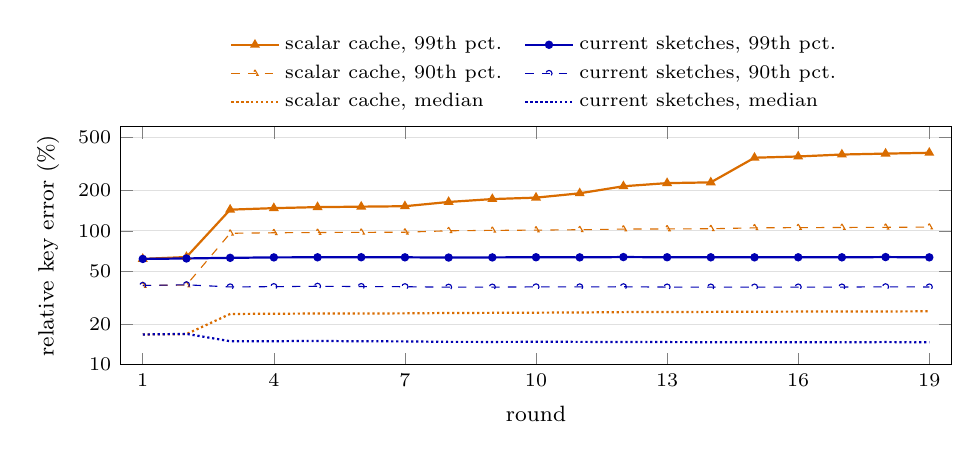
\begin{tikzpicture}
\begin{axis}[
  width=\columnwidth, height=4.6cm,
  ymode=log, ymin=10, ymax=600, xmin=0.5, xmax=19.5,
  xlabel={round}, ylabel={relative key error (\%)},
  xtick={1,4,7,10,13,16,19},
  ytick={10,20,50,100,200,500}, yticklabels={10,20,50,100,200,500},
  tick label style={font=\scriptsize}, label style={font=\footnotesize},
  ymajorgrids, grid style={black!12},
  legend style={font=\scriptsize,at={(0.5,1.03)},anchor=south,
    draw=none,inner sep=1pt,legend columns=2,
    /tikz/every even column/.append style={column sep=6pt}},
  legend cell align=left]
\addplot[orange!85!black,thick,mark=triangle*,mark size=1.3pt] coordinates {(1,61.73) (2,63.78) (3,144.23) (4,148.05) (5,150.67) (6,151.83) (7,153.03) (8,164.67) (9,173.09) (10,177.37) (11,191.19) (12,215.82) (13,227.89) (14,230.70) (15,352.94) (16,360.52) (17,372.88) (18,378.72) (19,384.24)};
\addlegendentry{scalar cache, 99th pct.}
\addplot[blue!70!black,thick,mark=*,mark size=1.1pt] coordinates {(1,61.73) (2,62.22) (3,62.90) (4,63.37) (5,63.48) (6,63.56) (7,63.46) (8,63.22) (9,63.36) (10,63.54) (11,63.40) (12,63.74) (13,63.53) (14,63.48) (15,63.45) (16,63.49) (17,63.45) (18,63.73) (19,63.43)};
\addlegendentry{current sketches, 99th pct.}
\addplot[orange!85!black,dashed,mark=triangle,mark size=1.3pt] coordinates {(1,39.08) (2,39.38) (3,96.00) (4,96.85) (5,97.29) (6,97.56) (7,97.81) (8,100.26) (9,100.92) (10,101.40) (11,102.06) (12,103.20) (13,103.50) (14,103.82) (15,105.41) (16,105.82) (17,106.09) (18,106.40) (19,106.73)};
\addlegendentry{scalar cache, 90th pct.}
\addplot[blue!70!black,dashed,mark=o,mark size=1.1pt] coordinates {(1,39.08) (2,39.53) (3,38.10) (4,38.30) (5,38.54) (6,38.36) (7,38.24) (8,37.93) (9,37.98) (10,38.13) (11,38.13) (12,38.20) (13,38.01) (14,38.01) (15,38.00) (16,38.02) (17,38.01) (18,38.20) (19,38.07)};
\addlegendentry{current sketches, 90th pct.}
\addplot[orange!85!black,densely dotted,thick] coordinates {(1,16.80) (2,16.91) (3,23.91) (4,24.02) (5,24.09) (6,24.13) (7,24.16) (8,24.31) (9,24.38) (10,24.46) (11,24.53) (12,24.69) (13,24.74) (14,24.79) (15,24.87) (16,24.91) (17,24.94) (18,24.98) (19,25.03)};
\addlegendentry{scalar cache, median}
\addplot[blue!70!black,densely dotted,thick] coordinates {(1,16.80) (2,16.97) (3,14.96) (4,14.96) (5,15.02) (6,14.94) (7,14.91) (8,14.79) (9,14.78) (10,14.80) (11,14.79) (12,14.76) (13,14.73) (14,14.71) (15,14.68) (16,14.69) (17,14.68) (18,14.73) (19,14.68)};
\addlegendentry{current sketches, median}
\end{axis}
\end{tikzpicture}
\caption{HepPh, $d=64$: relative error of the estimated key $r_2/r_1$
against exact moments before each round, over all active candidates
(mean of five projection draws). The scalar cache keeps its initial
absolute error; the current sketches used by \alg{} for unrefreshed
candidates keep a constant relative error.}
\label{fig:errtraj}
\end{figure}

Sketch-only removes retention. It takes 424 seconds on YouTube and
570 on Skitter, versus 113 and 297 for \alg{}, with nearly identical
trace estimates. On Skitter, 12 of 19 hybrid rounds need no refresh;
only 128 candidates are ever refreshed. Independent sketch-only
results cover these two graphs and roadNet-PA; missing cells are
shown explicitly. LiveJournal's completed scalar-cache set was not
evaluated. The cap-64 roadNet-PA sketch-only result is discussed below.

\begin{table}[t]
\centering\footnotesize
\caption{Four further seeds of the selection randomness, $K=20$,
$d=64$, fixed common seed vertex: mean $\pm$ standard deviation of
selection time (s) and of the paired gap
$(\widehat\Phi_1(\text{ApproxGreedy})-\widehat\Phi_1(\alg{}))/\widehat\Phi_1$;
The last column gives the range of per-seed paired gap/SE ratios.}\label{tab:seeds5}
\setlength{\tabcolsep}{2pt}
\begin{tabular}{@{}lrrrrr@{}}\toprule
Graph & \alg{} & ApproxGreedy & Speedup & Gap (\%) & Gap/SE\\\midrule
DBLP & $37.6\pm3.4$ & $123.9\pm2.3$ & $3.29\times$ & $0.035\pm0.009$ & 3.4--5.5\\
Amazon & $136.2\pm9.2$ & $189.6\pm8.8$ & $1.39\times$ & $0.219\pm0.047$ & 5.4--10.0\\
YouTube & $156.0\pm19.6$ & $585.5\pm41.8$ & $3.75\times$ & $0.019\pm0.010$ & 0.7--8.1\\
roadNet-PA & $343.5\pm7.9$ & $793.6\pm18.8$ & $2.31\times$ & $1.191\pm0.078$ & 5.8--7.5\\
\bottomrule\end{tabular}
\end{table}

\subsection{Sensitivity to budget, dimension, and refresh cap}\label{sec:sensitivity}
We vary $K$, $d$, and $b_r$ to test the balance between reuse,
estimate quality, and refinement work. Tables~\ref{tab:ksweep}
and~\ref{tab:dsweep} vary one parameter at a time on DBLP,
YouTube, and roadNet-PA; refresh totals count distinct candidates.

\begin{table}[t]
\centering\footnotesize
\caption{Total budget $K$ ($d=64$): selection time (s) and paired
difference $\widehat\Phi_1(\text{ApproxGreedy})-\widehat\Phi_1(\alg{})$
$\pm$ SE; positive values favor \alg{}.}\label{tab:ksweep}
\setlength{\tabcolsep}{3.5pt}
\begin{tabular}{@{}lrrrrr@{}}\toprule
Graph & $K$ & \alg{} & ApproxGreedy & Speedup & Difference\\\midrule
DBLP & 10 & 24.3 & 49.2 & $2.0\times$ & $+23.8\pm12.2$\\
 & 20 & 42.1 & 115 & $2.7\times$ & $+97.2\pm16.7$\\
 & 50 & 92.7 & 402.6 & $4.3\times$ & $+160.0\pm17.3$\\\midrule
YouTube & 10 & 56.1 & 237.4 & $4.2\times$ & $+65.5\pm32.7$\\
 & 20 & 112.9 & 646 & $5.7\times$ & $+241.7\pm44.3$\\
 & 50 & 346.7 & 2260.3 & $6.5\times$ & $+349.8\pm43.5$\\\midrule
roadNet-PA & 10 & 160.1 & 333.6 & $2.1\times$ & $+48575\pm10477$\\
 & 20 & 355.8 & 795 & $2.2\times$ & $+51513\pm5865$\\
 & 50 & 1020.4 & 2590.4 & $2.5\times$ & $+18562\pm3366$\\
\bottomrule\end{tabular}
\end{table}

\begin{table}[t]
\centering\footnotesize
\caption{Selection sketch dimension $d$ ($K=20$): selection time
(s), distinct refreshed candidates, and paired difference
$\widehat\Phi_1(d)-\widehat\Phi_1(64)\pm$ SE.}\label{tab:dsweep}
\setlength{\tabcolsep}{3pt}
\begin{tabular}{@{}lrrrr@{}}\toprule
& $d=16$ & $d=32$ & $d=64$ & $d=128$\\\midrule
DBLP time & 56.9 & 46.3 & 42.1 & 38.7\\
\quad refreshes & 512 & 368 & 256 & 176\\
\quad difference & $+50.7\pm8.8$ & $+4.3\pm10.4$ & -- & $-4.7\pm9.2$\\\midrule
YouTube time & 406.7 & 240.8 & 112.9 & 115.6\\
\quad refreshes & 784 & 448 & 144 & 96\\
\quad difference & $+254.9\pm45.9$ & $+160.1\pm33.3$ & -- & $+21.3\pm39.5$\\\midrule
roadNet-PA time & 314.8 & 324.2 & 355.8 & 365.1\\
\quad refreshes & 304 & 304 & 304 & 304\\
\quad difference & $+58297\pm6725$ & $+22505\pm5047$ & -- & $-9086\pm4940$\\
\bottomrule\end{tabular}
\end{table}

\paragraph{Budget}
More rounds increase the opportunity for reuse. From $K=10$ to
$K=50$, the speedup over ApproxGreedy rises from $2.0\times$ to
$4.3\times$ on DBLP and $4.2\times$ to $6.5\times$ on YouTube;
it remains $2.1$--$2.5\times$ on roadNet-PA. \alg{} has lower
estimated inverse trace at every tested budget. The gaps exceed
four SE except at $K=10$ on DBLP and YouTube, where they are
about two SE.

\paragraph{Sketch dimension}
A narrower solution sketch can increase refinement cost. Raising $d$ from 16
to 64 reduces YouTube's refreshes from 784 to 144 and time from
407 to 113 seconds; DBLP shows the same pattern. At $d=128$,
trace differences from $d=64$ are within two SE on all three graphs.
On roadNet-PA the cap binds throughout the sweep, and time instead
rises mildly with dimension, from 315 to 365 seconds.

\paragraph{Refresh cap}
The cap trades refinement against quality. On roadNet-PA,
sketch-only caps 16 and 64 take 278 and 1069 seconds, reaching
$3.2366\times10^6$ and $3.2098\times10^6$. The hybrid with cap
16 lies between them in quality, at $3.2230\times10^6$ in 356
seconds. On Skitter the cap is inactive. These cases separate
bounded refinement from the benefits of the two update paths.

\begin{table*}[t]
\centering\footnotesize
\caption{Exact-marginal lazy selection on medium graphs, $K=20$,
common seed, $\sigma=0$. Each entry is $\lambda_{\min}\,/\,\tr X^{-1}$,
evaluated exactly: the trace sums unit-vector solves at relative
residual $10^{-9}$, and $\lambda_{\min}$ is computed by Lanczos.
Zhou uses our Fast reimplementation.}
\label{tab:medium}
\setlength{\tabcolsep}{5pt}
\begin{tabular}{@{}lrrrrr@{}}\toprule
& HepPh & AstroPh & CondMat & CAIDA & Enron\\
$n\,/\,m$ & 11,204 / 117,619 & 17,903 / 196,972 & 21,363 / 91,286 & 26,475 / 53,381 & 33,696 / 180,811\\\midrule
$p=1$ & .0639 / 4329.56 & .0485 / 4428.97 & .0274 / 8874.27 & .0656 / 18909.45 & .0557 / 17675.78\\
$p=2$ & .0845 / 4332.34 & .0841 / 4432.76 & .0427 / 8888.70 & .0967 / 18915.01 & .0759 / 17679.66\\
$p=3$ & .0991 / 4337.35 & .0996 / 4437.98 & .0506 / 8905.52 & .0964 / 18916.07 & .0759 / 17679.75\\
$p=4$ & .0991 / 4338.33 & .1127 / 4444.54 & .0574 / 8927.88 & .0990 / 18919.00 & .0887 / 17686.85\\
$p=8$ & .1165 / 4358.79 & .1193 / 4465.39 & .0660 / 8966.20 & .1068 / 18927.34 & .0887 / 17700.28\\
Zhou & .1096 / 4343.63 & .1127 / 4443.31 & .0604 / 8935.30 & .1037 / 18921.59 & .0888 / 17690.66\\
\bottomrule\end{tabular}
\end{table*}

\begin{figure*}[t]
\centering
\begin{tikzpicture}
\begin{groupplot}[
  group style={group size=5 by 1, horizontal sep=10mm},
  scale only axis, width=2.55cm, height=2.2cm,
  tick label style={font=\tiny}, title style={font=\scriptsize,yshift=-4pt},
  label style={font=\scriptsize},
  enlarge x limits=0.14, enlarge y limits=0.14, clip=false,
  scaled ticks=false, xticklabel style={/pgf/number format/fixed,
    /pgf/number format/1000 sep={}},
  yticklabel style={/pgf/number format/fixed,/pgf/number format/precision=3},
  max space between ticks=40]
\nextgroupplot[title={HepPh}, ylabel={$\lambda_{\min}$}]
\addplot[blue!70!black,mark=*,mark size=1.3pt] coordinates {(4329.56,0.0639) (4332.34,0.0845) (4337.35,0.0991) (4338.33,0.0991) (4358.79,0.1165)};
\addplot[only marks,orange!85!black,mark=triangle*,mark size=2.2pt] coordinates {(4343.63,0.1096)};
\node[font=\tiny,anchor=west] at (axis cs:4329.56,0.0639) {1};
\node[font=\tiny,anchor=north west] at (axis cs:4358.79,0.1165) {8};
\nextgroupplot[title={AstroPh}]
\addplot[blue!70!black,mark=*,mark size=1.3pt] coordinates {(4428.97,0.0485) (4432.76,0.0841) (4437.98,0.0996) (4444.54,0.1127) (4465.39,0.1193)};
\addplot[only marks,orange!85!black,mark=triangle*,mark size=2.2pt] coordinates {(4443.31,0.1127)};
\node[font=\tiny,anchor=west] at (axis cs:4428.97,0.0485) {1};
\node[font=\tiny,anchor=north west] at (axis cs:4465.39,0.1193) {8};
\nextgroupplot[title={CondMat}]
\addplot[blue!70!black,mark=*,mark size=1.3pt] coordinates {(8874.27,0.0274) (8888.7,0.0427) (8905.52,0.0506) (8927.88,0.0574) (8966.2,0.066)};
\addplot[only marks,orange!85!black,mark=triangle*,mark size=2.2pt] coordinates {(8935.3,0.0604)};
\node[font=\tiny,anchor=west] at (axis cs:8874.27,0.0274) {1};
\node[font=\tiny,anchor=north west] at (axis cs:8966.2,0.066) {8};
\nextgroupplot[title={CAIDA}]
\addplot[blue!70!black,mark=*,mark size=1.3pt] coordinates {(18909.45,0.0656) (18915.01,0.0967) (18916.07,0.0964) (18919.0,0.099) (18927.34,0.1068)};
\addplot[only marks,orange!85!black,mark=triangle*,mark size=2.2pt] coordinates {(18921.59,0.1037)};
\node[font=\tiny,anchor=west] at (axis cs:18909.45,0.0656) {1};
\node[font=\tiny,anchor=north west] at (axis cs:18927.34,0.1068) {8};
\nextgroupplot[title={Enron}]
\addplot[blue!70!black,mark=*,mark size=1.3pt] coordinates {(17675.78,0.0557) (17679.66,0.0759) (17679.75,0.0759) (17686.85,0.0887) (17700.28,0.0887)};
\addplot[only marks,orange!85!black,mark=triangle*,mark size=2.2pt] coordinates {(17690.66,0.0888)};
\node[font=\tiny,anchor=west] at (axis cs:17675.78,0.0557) {1};
\node[font=\tiny,anchor=north west] at (axis cs:17700.28,0.0887) {8};
\end{groupplot}
\node[font=\scriptsize] at ($(group c1r1.south west)!0.5!(group c5r1.south east)+(0,-0.75)$) {$\tr X^{-1}$ (lower is better)};
\end{tikzpicture}
\caption{CFCC/spectral tradeoff on the medium graphs of
Table~\ref{tab:medium}. Circles join the sets selected at
$p=1,2,3,4,8$ (labels mark $p=1$ and $p=8$); the triangle is Zhou's
single set.}
\label{fig:tradeoff}
\end{figure*}

\begin{table}[t]
\centering\footnotesize
\caption{Paired-probe differences $\widehat\Phi_1(\cdot)-\widehat\Phi_1(\alg{})$
on the final sets of Table~\ref{tab:main} (128 common probes), with
standard errors of the difference. Positive values favor \alg{};
roadNet-PA entries are in thousands.}\label{tab:paired}
\setlength{\tabcolsep}{2pt}
\begin{tabular}{@{}lrrrr@{}}\toprule
Graph & ApproxGreedy & ForestCFCM & SchurCFCM & Zhou\\\midrule
DBLP & $+97.2\pm16.7$ & $+553.5\pm30.3$ & $+122.5\pm14.2$ & $+448\pm33$\\
Amazon & $+266.9\pm47.6$ & $+1149.6\pm74.5$ & $-164.5\pm47.6$ & $+749\pm85$\\
YouTube & $+241.7\pm44.3$ & $+2637.2\pm81.4$ & $-37.4\pm44.8$ & $-10.5\pm39$\\
web-Google & $+404\pm79$ & $+3247.3\pm143.2$ & $+302.4\pm83.5$ & $+661\pm98$\\
Skitter & $+28.8\pm22$ & $+2001.9\pm66.9$ & $+434.6\pm29.5$ & $-43.1\pm19.6$\\
roadNet-PA & $+51.5\pm5.9$ & $-17.0\pm5.8$ & $-23.8\pm5.8$ & $+22.2\pm5.6$\\
\bottomrule\end{tabular}
\end{table}

\subsection{Variability and paired differences}\label{sec:variability}
Selection randomness and evaluation noise measure different sources
of variation. Table~\ref{tab:seeds5} uses four further selection
seeds (1001--1004) with a fixed initial anchor. Population standard deviations
summarize these runs; speedups are ratios of mean times.
\alg{} remains faster on all four graphs, by $1.39$--$3.75\times$,
and has lower estimated inverse trace in all 16 graph--seed pairs.
Fifteen paired gaps exceed three SE; the remaining YouTube pair has
gap/SE $=0.7$.

Table~\ref{tab:paired} evaluates the main-run sets with common
probes to reduce noise in the differences. For example, the DBLP
comparison with ApproxGreedy has paired SE 16.7, versus 82 for a
single trace estimate. These paired errors support the main quality
comparisons; the repeated-selection standard deviations describe
run-to-run variation separately.

\subsection{The inverse power as a tunable knob}\label{sec:powers}
This experiment tests spectral weighting independently of the
large-scale $p=1$ sketch implementation. On five medium graphs,
exact-marginal lazy selection uses $p=1,2,3,4,8$, with moments
computed by numerical solves. Final traces use unit-vector solves
at relative residual tolerance $10^{-9}$, and smallest eigenvalues
use Lanczos (Table~\ref{tab:medium}, Fig.~\ref{fig:tradeoff}).

From $p=1$ to $p=4$, $\lambda_{\min}$ increases by
$1.51$--$2.33\times$, while inverse trace rises only 0.05--0.60\%.
Among the tested powers, $p=1$ gives the lowest trace on each graph.
The spectral response is not strictly monotone: CAIDA has a 0.4\%
dip from $p=2$ to $p=3$. At $p=4$, the smallest eigenvalue is
within 0.1\% of Zhou's on AstroPh and Enron, and 4.5--9.5\%
lower on the other graphs. At $p=8$, it exceeds Zhou's on four
graphs and is 0.05\% lower on Enron. These sets expose the cost
of emphasizing slower modes rather than treating either objective
as interchangeable with CFCC.

\section{Related Work}\label{sec:related}
\paragraph{Group centrality and grounded spectra}
Li et al.~\cite{li2019} formulate CFCC, establish optimization
hardness and reciprocal-objective supermodularity, and develop exact
and randomized greedy algorithms, including ApproxGreedy.
Current-flow closeness of single vertices goes back to Brandes and
Fleischer~\cite{brandes2005}, and group centralities to Everett and
Borgatti~\cite{everett1999}. Greedy and local-search maximization has
been engineered for shortest-path group closeness and group
harmonic centrality~\cite{bergamini2018,angriman2021}, group
betweenness by sampling~\cite{mahmoody2016}, and group forest
closeness~\cite{grinten2021}. Group Markov centrality considers
related hitting-time group objectives~\cite{wang2026}. Zhou et al.~\cite{zhou2023} instead
maximize the smallest grounded eigenvalue, establishing monotonicity
and failure of submodularity, and propose the Fast sensitivity score.
Aggregate resistance and the slowest spectral mode capture different
aspects of a selected group. Our CM formulation places CFCC in a
trace family with tunable inverse-power weighting and an explicit
connection to the spectral endpoint.

\paragraph{Leader selection}
In networked control, choosing $k$ noise-free leaders to minimize the
steady-state variance of consensus followers is the same grounded
inverse-trace problem~\cite{patterson2010}. Clark et
al.~\cite{clark2014} prove its supermodularity and analyze greedy
selection; Lin et al.~\cite{lin2014} give convex relaxations and
bounds. These methods use dense inverses and target networks of
hundreds to thousands of nodes. The smallest eigenvalue of the
grounded Laplacian, which governs convergence to the leaders, is
analyzed by Pirani and Sundaram~\cite{pirani2016}.

\paragraph{Forest sampling for CFCC}
Xia and Zhang~\cite{xia2025} estimate CFCC marginals using spanning
forests rooted at the selected group and generated by Wilson's
algorithm~\cite{wilson1996}. ForestCFCM estimates marginals directly;
SchurCFCM introduces auxiliary high-degree roots and applies
Schur-complement corrections. Both draw new forests after each
selection and use graph-dependent bounds for adaptive sampling.
\alg{} instead maintains solution sketches across grounding updates
and retains refreshed moments, reducing repeated all-candidate
estimation.

\paragraph{Spectral design and matrix functions}
FastFrac~\cite{fastfrac} optimizes positive fractional traces under
edge addition; POLAR~\cite{polar} studies negative fractional
objectives through submodularity-ratio analysis. Edge modification
changes walk transition rates, whereas grounding changes survival by
killing or removing active coordinates. Matrix-function representations
and quadrature~\cite{golub2010} evaluate spectral objectives through
resolvents. Our integer formulation uses inverse moments for finite
grounding marginals and their incremental updates.

\paragraph{Randomized and incremental numerical methods}
JL projections reduce inverse-diagonal estimation to a small number
of solves, as in effective-resistance sketching~\cite{ss2011} and
ApproxGreedy~\cite{li2019}. Sherman--Morrison
identities~\cite{sherman1950} give rank-one inverse updates, while
classical lazy greedy~\cite{leskovec2007} uses stale submodular
upper bounds. \alg{} combines current sketches, retained moments,
and capped refresh; its analysis handles reuse of the same
projections across adaptive rounds. Nearly-linear solvers and sparse
elimination~\cite{spielman2014,kyng2016} provide the numerical
primitives.

\begin{samepage}
\section{Conclusion}
\alg{} reduces repeated CFCC estimation by updating solution sketches
and retaining refreshed moments. Its seeded-gain analysis makes
adaptive sampling and numerical conditions explicit. The measurements
show both substantial solve savings and limits from
maintenance or refresh work, with input-dependent quality tradeoffs.
The CM and inverse-power extension supplies a separate choice of
spectral objectives.
\par\end{samepage}

\section*{Acknowledgment}
Generative AI tools, including OpenAI ChatGPT/Codex and Anthropic
Claude, assisted with drafting and revising prose throughout the
manuscript and implementing experiment code for Section~VI.
They also helped develop parts of the proofs and counterexample
analysis in Sections~II--V, based on the authors' ideas and
preliminary verification approaches. The authors reviewed the AI-assisted
content, checked its accuracy, and take full responsibility
for the final manuscript.
